\documentclass[a4paper]{scrartcl}

%\usepackage[applemac]{inputenc}
\usepackage[utf8]{inputenc}
%\usepackage{a4wide}
\usepackage{graphicx}
\usepackage{tabularx}
\usepackage{pstricks-add}
\usepackage{url}
\usepackage{auto-pst-pdf}
\usepackage[english]{babel}
\usepackage{hyperref}[2010/09/11]

% Kopf- und Fusszeilen
\usepackage{fancyhdr}
\pagestyle{fancy}
\fancyhead{}
\fancyfoot{}
\lhead{HSR University of Applied Science Rapperswil}
\rhead{Term Project}
\lfoot{\copyright \ Nicolas Bigler, Michael Fisler}
\rfoot{Page \thepage}
\renewcommand{\headrulewidth}{0.4pt} 
\renewcommand{\footrulewidth}{0.4pt}


\title{
	\vspace{-30mm}
	\hspace{-40mm}
	
\includegraphics{Bilder/HSR_Logo_CMYK.eps}
	\newline
	\newline
	\newline
	\newline
	\newline
	\newline
	\newline
%\fbox{\textwidth}{
Validation of the Background Radiation Detector
%}
 \\ \ \\ Term Project \\ \ \\ \ }
\subtitle{
	Department of Computer Science \\ University of Applied Science Rapperswil \\ \ \\ \ Fall Term 2011\\ \ \\ \ \\ \ \\ \ \\ \ \\ \ 
}

\author{
Authors: Nicolas Bigler, Michael Fisler  \and
Advisor: Prof. Eduard Glatz \and		
Project Partner: - \and
External Co-Examiner: ? \and
Internal Co-Examiner: ?
}

%Suppress Date on Title Page
\date{}

% Absatzeinzug aufheben
\parindent 0pt

% Set Paragraph Spacing
\parskip 6pt

\begin{document}

%Marginals on the left Side 
\reversemarginpar
\maketitle
\newpage
\tableofcontents
\newpage
\listoffigures
\newpage
%\listoftables
%\newpage

\section{Task}
A \marginpar{Starting position} substantial part of the internet's traffic stems from misconfiguration, worms, malware, viral activity or all sorts of attacks and therefore is undesirable. As this kind of traffic is constantly present it often is referred to as ``internet background radiation''. The monitoring of the background radiation yields valuable information in terms of malicious activity and may be used to predict future trends.

At ETH Zurich a tool was developed to distinguish between one-way and two-way flows and subsequently classify one-way traffic using a set of predefined rules.

Until now the available data was limited since only packet headers were recorded. It was therefore difficult to successfully validate the Background Radiation Detector due to the lack of information.

To gain more Information a special infrastructure was set up at HSR to record the entire traffic within a five day span in order to enable a more thorough validation. In addition to the packet headers and flow data the new infrastructure provides payloads from one-way flows and intrusion detection system (IDS) alerts.

Through\marginpar{Mission} analysis of the collected data skillfully using and combining different analysis methods the rules used by the detector shall be validated and optimized. As far as possible the validation shall be automated. The goal is to determine the false negative (FN) and false positive (FP) rates for each class.
The methods to use are as follows:
\begin{itemize}
	\item analysis of the state sequence (flag sequence, TCP packets only)
	\item analysis of the network management information data (ICMP packet analysis)
	\item correlation of IDS alerts and flow data
\end{itemize}

The main focus of this validation is on the classes ``malicious scanning'' (rule 5), ``suspicious other'' (rules 6 to 8), ``backscatter'' (rules 9 to 11) and ``suspected benign'' (rule 15). Class ``Bogon'' needs no validation.

The original text of the task (in German) is enclosed in the appendix [ref?].
\newpage

\section{Abstract}

\section{Management Summary}
The\marginpar{Starting position} goal of this project is the validation of the ``Background Radiation Detector'' which was developed at ETH Zurich. In a first step the detector identifies one-way flows and in a second step classifies those flows using predefined rules. In order to validate these rules and if necessary adapt them packet and flow data was recorded in a five day period. Additionally an intrusion detection system has been set-up to further investigate the cause of all incoming traffic.

Since\marginpar{Approach} we are dealing with very large PCAP files loading an entire file in Wireshark takes at least half an hour. In order to reduce the file size and thus allowing a more efficient manual analysis one-way flows from the original PCAP traces were written into new files according to the class they belong to.


blub \marginpar{Results} blub

blub \marginpar{Outlook} blub

\section{Technical Report}

\subsection{Infrastructure}
Data was collected between ... and ... on a server (``Collector'') connected between HSR's gateway and firewall.  The ``Collector'' is equipped with a high performance DAG Endace network card which allows to capture all packets even at full line rate. Using external time references the captured packet's timestamps are highly accurate. \cite{endace}. Attached to the collecting server a second server (``Analyzer'') is used to process and evaluate the data captured. It hosts an environment to compile and run validation software and tools such as Wireshark for further analysis.
\begin{figure}[ht]
	\begin{center}
		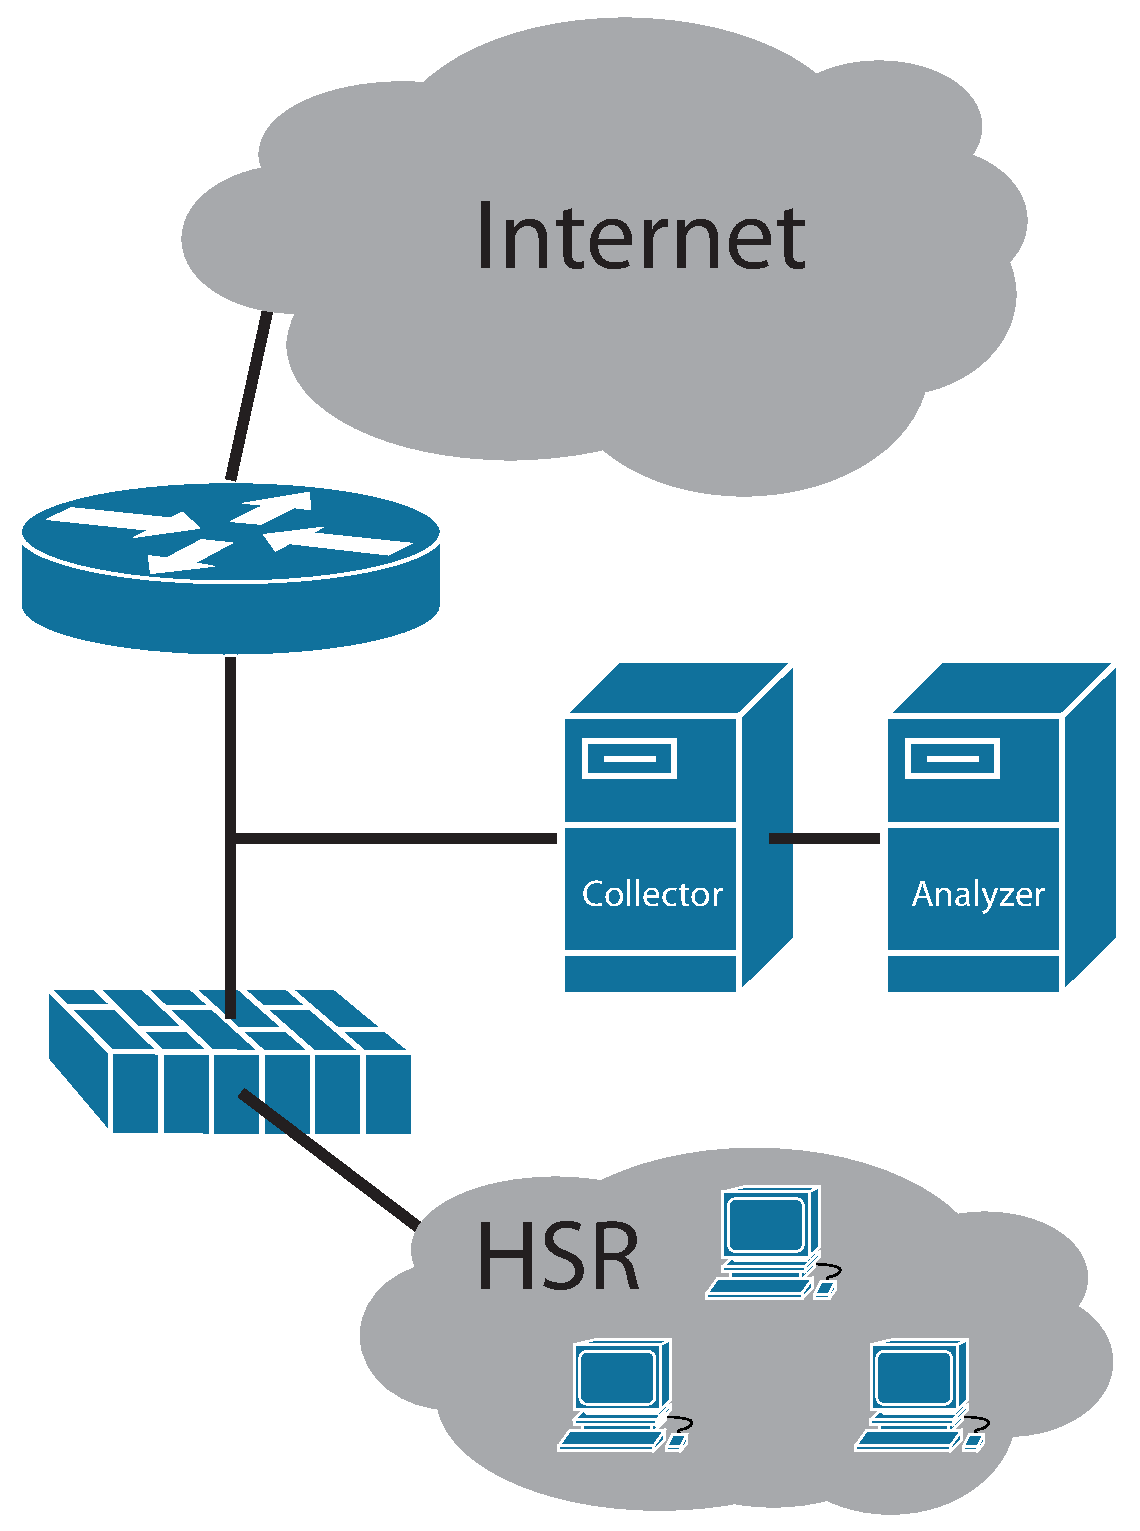
\includegraphics[width=200pt, keepaspectratio=true]{Bilder/Infrastruktur.eps}
		\caption{Validation infrastructure}
		\label{infra}
	\end{center}
\end{figure}

\subsection{Data}
The\marginpar{PCAP} validation is primarily based on PCAP traces which contain the entire traffic from and to the HSR in a five day span. The traces are split into one hour intervals. HSR is connected to the Switch network which doesn't filter traffic. We therefore get a good sample of the internet background radiation [quote Prof. Glatz].

Flow \marginpar{Flow data} data was generated from the PCAP files with YAF \cite{yaf} and converted from IPFIX to CFlow format. The resulting files contain flow data in 10 minute intervals. Each flow is defined by its starting time, its duration (which may exceed 10 minutes), the IP data and the flow direction. Only incoming flows (infl) and incoming flows which have a corresponding two-way flow with the same IP addresses and ports (q\_infl) are relevant for our validation.

Based\marginpar{Sign sets} on the flow data  Flow Daten wurden anschliessend mit dem O/W Classifier [] den verschiedenen Klassen zugeordnet. Als Resultat liegen Signdaten vor in denen die Klassenzugehörigkeit der Flows gespeichert ist.

In\marginpar{IDS alerts} addition to the flow and sign data, alerts generated by the open-source intrusion detection system Snort can be used to investigate the intent of the flows. In order to be able to correlate these alerts with the packet and flow data, the same anonymizing scheme was used.

\subsubsection{Data privacy}
In order to meet the data privacy requirements at HSR all IP addresses are anonymized and all data above the transport layer has been stripped from packets belonging to two-way flows. Layer 4 PDU are available for one-way flows only. The anonymization generates random IP addresses but preserves prefixes (i.e. subnet membership is preserved). It therefore is impossible to identify the hosts, networks oder services behind those IP addresses. As a consequence it is very difficult to figure out if a certain host is a regular server and neither the geographic location, nor the provider who owns the respective IP address can be identified. We discovered that the IP addresses 152.103.xxx.xxx are HSR addresses since they were present in almost all packets.

\subsubsection{Limitations of our flow data}
YAF has some limitations in terms of flow defragmentation. If a connection is terminated with a FIN flag and packets are retransmitted after that, YAF interprets those retransmissions as independent one-way flows. The same holds true if Multiple RST packets are sent. HOW MANY?

\subsection{Basic Validation Concepts}
In\marginpar{TCP} case of TCP one-way flows the only valid flag sequence is a sequence of multiple SYN flags. If only one SYN flag is sent we consider that to be a SYN scan because benign applications should try to establish a connection more than once if they don't receive a SYN/ACK. Most applicaitons use the default socket and therefore do that by default [quote Prof. Glatz]. Before a connection is established RFC 793 \cite{rfc_tcp} forbids the use of flags other than SYN. 

To\marginpar{UDP} validate UDP flows we use the UDP PDU's size. Packets without a payload are a priori suspicious. Regular UDP packets should at least contain protocol headers from OSI layers 5 to 7 even if no user data is sent and therefore contain a UDP PDU.
In addition to the existence of a PDU the variance of size over all packets within the flow may be used to identify malicious intent. If all PDUs are the same size the flow is certainly not a regular benign flow but rather a scan. BRINGT DIESES KRITERIUM ETWAS? AUSWERTUNG ANSCHAUEN!!!

\subsection{Flow Classes}
In this section we describe the classes that need to be validated. All descriptions are from a validation perspective, for details and rules refer to [Glatz'sche publikation, bzw. Auszug]. The classification currently used by the background radiation detector is based on seven disjoint classes. Provided that all flows can be assigned to the proper class false negative and false positive rates can therefore be calculated. In addition to the description of each class our strategies for the validation of each class are layed out.

\begin{figure}[ht]
\begin{center}
\psset{framesep=1.1pt,unit=1.1cm}
\begin{pspicture}(-5.1,-5.1)(5.1,5.1)
	\degrees[100]
	\pswedge[fillstyle=hlines,fillcolor=gray,hatchcolor=gray]{5}{ 0 }{65.24 }
	\rput(4.2; 32.62 ){\psframebox*{\small 65.24 \%}}
	\uput{5.2}[ 32.62 ](0;0){\small Malicious Scanning}
	\pswedge[fillstyle=hlines,fillcolor=gray,hatchcolor=gray]{5}{65.24 }{93.16 }
	\rput(4.2;79 ){\psframebox*{\small 27.92 \%}}
	\uput{5.2}[79 ](0;0){\small Suspicious Other}
	\pswedge[fillstyle=hlines,fillcolor=gray,hatchcolor=gray]{5}{93.16 }{95.39 }
	\rput(4.2;94.2 ){\psframebox*{\small 2.23 \%}}
	\uput{5.2}[94.2 ](0;0){\small Backscatter}
	\pswedge[fillstyle=solid,fillcolor=white,hatchcolor=white]{5}{95.39 }{95.52 }
%	\rput(4.2;95.4 ){\psframebox*{\small 0.13 \%}}
	\uput{5.2}[95.4 ](0;0){\small Serv. Unreach. (0.13 \%)}
	\pswedge[fillstyle=solid,fillcolor=white,hatchcolor=white]{5}{95.52 }{98.49 }
	\rput(4.2;97 ){\psframebox*{\small 2.97 \%}}
	\uput{5.2}[97 ](0;0){\small P2P Scanning}
	\pswedge[fillstyle=solid,fillcolor=white,hatchcolor=white]{5}{98.49 }{98.68 }
%	\rput(4.2;98 ){\psframebox*{\small 0.19 \%}}
	\uput{5.2}[98 ](0;0){\small Susp. Benign (0.19 \%)}
	\pswedge[fillstyle=solid,fillcolor=gray,hatchcolor=gray]{5}{98.68 }{98.94 }
%	\rput(4.2;98.7 ){\psframebox*{\small 0.26 \%}}
	\uput{5.2}[98.7 ](0;0){\small Bogon (0.26 \%)}
	\pswedge[fillstyle=solid,fillcolor=gray,hatchcolor=gray]{5}{98.94 }{100 }
	\rput(4.2;99.5 ){\psframebox*{\small 1.8 \%}}
	\uput{5.2}[99.5 ](0;0){\small Other}
\end{pspicture}
\caption{Classes as used by the ``O/W Classifier''.  95.93\% of all flows were identified as malign (striped), 3.29\% benign (white) and 2.06\% not defined (grey).}
		\label{class}
	\end{center}
\end{figure}

\subsubsection{Malicious Scanning}

All \marginpar{Character\-istics} malicious scan activities as well as traffic generated by viruses, trojans and worms are summarized in this class. With the exception of SYN scans, the length of the flows is basically not limited. It is definitely  possible that a flow contains multiple packets from different scans. UDP scans normally have a specific payload depending on the destination service. \cite{nmap09}.

For \marginpar{Validation} the validation of TCP flows the scan patterns of NMAP are used \cite{nmap09}:
\begin{itemize}
	\item Christmas Scan:  Packets with flags FIN, PSH and URG set.
	\item Null Scan: A packet without any TCP flags set is sent without an established TCP connection. 
	\item FIN Scan: A packet with the FIN flag is sent without an established TCP connection.
	\item SYN Scan: A single packet with the SYN flag set is being sent.
\end{itemize}
With those criteria the true positive rate can be determined. 
To ascertain the false positive rate, the TCP flows that could not be clearly verified as scan, are manually checked for their class affiliation.

For the analysis of ICMP flows we use the fact, that scanning is only possible with ICMP requests, because all other ICMP messages are not acknowledged\cite{rfc_icmp}. Therefore the false positive rate of the ICMP flows adds up to the number of ICMP responses.

\subsubsection{Suspicious Other}
This\marginpar{Character\-istics} class containts all flows that could not be assigned to the remaining classes ``Malicious Scanning'' and ``Backscatter'', but probably have malicious origin.

All\marginpar{Validation} TCP flows that do not have a valid flow sequence should a priori be classified as malicious. If a valid flow sequence is present, it is not possible to classify the flow without further information, because malicious scans can also use valid sequences as a camouflage. \cite{nmap09}.

\subsubsection{Backscatter}
Backscatter\marginpar{Character\-istics} is incoming traffic caused by attacks to hosts in other networks with faked source addresses. The received replies to those attacks are called backscatter[]. 

ICMP\marginpar{Validation} packets triggered by backscatter scanning can only be replies, because backscatter is always a reaction to faked incoming packets from another network. Possible requests thus fall into the category false positive.

TCP flows cannot contain SYN flags, because they initiate connection and therefore cannot be backscatter. The flag sequences in the class backscatter have to be valid as defined in the TCP state machine \cite{rfc_tcp} because the origin of these packets are regular hosts and network devices. <-- UMSETZEN!

\subsubsection{Service Unreachable}
``Service Unreachable''\marginpar{Character\-istics} contains all flows, that are generated <bad choice of word!> because of temporarily unavailable services.

One\marginpar{Validation} approach is to check if the destination address resides on an unused range of the HSR. If this is the case

Since HSR does not suppress outgoing ICMP destination unreachable packets, such packets may be used to identify unreachable services. To match ICMP packets with flows classified as ``Service Unreachable'' the IP and port information from the ICMP packet's payload \cite{rfc_icmp} can be used. 

\subsubsection{Benign P2P Scanning}
``Benign P2P Scanning''\marginpar{Charakter\-istics} contains all flows which originate from P2P applications scanning for currently unavailable peers.

As\marginpar{Validierung} a mean to validate this class the packets payload can be checked for the existence of a P2P protocol header. Due to the capability of modern P2P applications to obfuscate \cite{emule} or encrypt \cite{vuze} traffic there will be a remainder of unknown cause.

\subsubsection{Suspected Benign}
``Suspected Benign''\marginpar{Charakter\-istics} contains all traffic which is considered benign and has not been classified as ``P2P'' or ``Service Unreachable''. As an example one-way flows which were caused by misconfiguration fall in this class.

As\marginpar{Validation} a remainder class the validation hinges on the definition of ``benign flow''. 
In order to avoid a formal and possibly flawed definition we try to detect malicious patterns to gauge the false positive rate.
In case of TCP flows we define flows that contain an invalid flag sequence malign. On one hand benign applications should follow the TCP state machine defined in RFC793 \cite{rfc_tcp}, on the other hand most applications use the default socket and therefore implement the state machine by default. [quote Prof. Glatz]
In any case snort alerts may be used to verify the intent of each flow not confirmed as malign.

\subsubsection{Bogon}
Class ``Bogon'' was not validated and therefore will not go into details.

\subsubsection{Other}
``Other'' contains all flows which could not successfully be assigned to one of the before mentioned classes. It is not a class in the narrower sense but a remainder class. Therefore neither true positive nor false negative rates can be determined.

The\marginpar{Validation} false positive rate is a result of all true positive criteria for each class.


\subsection{Results}
\subsubsection{Statistics per class}
\subsubsection{}
\subsection{Conclusions}

lorem ipsum...

\section{Appendix}

\subsection{Report Nicolas Bigler}

\subsection{Report Michael Fisler}

\subsection{Test Documentation}

\subsection{Meeting Protocols}
	\href{meeting\_protocols.pdf}{meeting\_protocols.pdf}

\subsection{Project Plan}
	\href{./project\_plan.pdf}{project\_plan.pdf}


\subsection{Task description}
%	\href{./task\_description.pdf}{task\_description.pdf}

%In Abbildung \ref{sc_kz} sind die Finanzkennzahlen 2010/2011 der Swisscom dargestellt%\cite{oppenheimer11}.


%In Tabelle \ref{plnp} sind die technischen Anforderungen aufgeführt:
%\begin{table}[h]
%\begin{tabularx}{\textwidth}{|l|X|}
%	\hline Skalierbarkeit & Option für Feeder Netzwerk (Bündelung und Multiplex);  \\ 
%	\hline Verfügbarkeit & Hoch: Silber: 99.95\%, Gold: 99.97\% \\
%	\hline Performanz & 2 - 155 Mbps \\
%	\hline Sicherheit & Hoch, physikalisch getrennte Leitungen, Farbe pro Kunde \\
%	\hline Verwaltung & Proaktives End-zu-End Management \\
%	\hline Anpassbarkeit & Schwierig anzupassen \\
%	\hline Erschwinglichkeit & Teuer, lohnt sich nur bei entsprechender Aulastung der Leitung, Granularität der Bandbreite schlecht \\
%	\hline
%\end{tabularx}
% \caption{Private Line National Plus Technische Anforderungen}
%	\label{plnp}
%\end{table}


\newpage
\begin{thebibliography}{9}

	\bibitem{nmap09} Gordon ``Fyodor'' Lyon, \emph{Nmap Network Scanning: The Official Nmap Project Guide to Network Discovery and Security Scanning},
	Nmap Project,
	2009
	
	\bibitem{icmp} IANA.org, Internet Control Message Protocol (ICMP) Parameters \\
	\url{http://www.iana.org/assignments/icmp-parameters/icmp-parameters.xml}
	
	\bibitem{rfc_tcp} IETF.org, RFC793: Transmission Control Protocol (TCP) \\
	\url{http://www.ietf.org/rfc/rfc793.txt}
	
	\bibitem{rfc_icmp} IETF.org, RFC792: Internet Control Message Protocol (ICMP) \\
	\url{http://www.ietf.org/rfc/rfc792.txt}
	
	\bibitem{emule} Emule-Project.net, Protocol Obfuscation \\
	\url{http://www.emule-project.net/home/perl/help.cgi?l=1&rm=show_topic&topic_id=848}
	
	\bibitem{vuze} Vuze.com, Message Stream Encryption \\
	\url{http://wiki.vuze.com/w/Message_Stream_Encryption}
	
	\bibitem{yaf} CERT.org, CERT NetSA Security Suite \\
	\url{http://tools.netsa.cert.org/yaf/}
	
	\bibitem{backscatter} CAIDA.org, Worldwide Detection of Denial of Service (DoS) Attacks \\
	\url{http://www.caida.org/publications/presentations/usenix0108/dos/dos.pdf}
	
	\bibitem{endace} Endace.com, Endace High Speed Capture Cards \\
	\url{http://www.endace.com/endace-dag-high-speed-packet-capture-cards.html}
	
\end{thebibliography}

\end{document}
